\documentclass[conference]{IEEEtran}
\IEEEoverridecommandlockouts
% The preceding line is only needed to identify funding in the first footnote. If that is unneeded, please comment it out.
\usepackage{gensymb}
\usepackage[spanish]{babel}
\usepackage[utf8]{inputenc}
\usepackage{cite}
\usepackage{amsmath,amssymb,amsfonts}
\usepackage{algorithmic}
\usepackage{graphicx}
\usepackage{textcomp}
\usepackage{xcolor}
\def\BibTeX{{\rm B\kern-.05em{\sc i\kern-.025em b}\kern-.08em
    T\kern-.1667em\lower.7ex\hbox{E}\kern-.125emX}}
\begin{document}

\title{Proyecto de investigación - Hilos.
\\
{\footnotesize\textsuperscript{Informática II}
}
}



\author{\IEEEauthorblockN{1\textsuperscript{st} Paubla Andrea Rivera Anaya}
\IEEEauthorblockA{\textit{Facultad de Ingeniería} \\
\textit{Universidad de Antioquia}\\
Medellín, Colombia \\
paubla.rivera@udea.edu.co}




}

\maketitle

\begin{abstract}

This report talks about threads, a feature that allows an application to multitask concurrently. Using these allows you to simplify the design of an application that must carry out different functions simultaneously. \\


\end{abstract}

\begin{IEEEkeywords}
Procesos, Roscado, Procesador, overhead, OS, API.
\end{IEEEkeywords}
\\
\\

\section{INTRODUCCIÓN}
\\
\\

Se ha dado gran importancia al desarrollo de algoritmos y programas que permitan resolver distintos problemas en cualquier campo que se requiera, por esta razón la implementación de hilos en un sistema operativo es indispensable, ya que estos aumentan la eficiencia de la comunicación entre programas en ejecución. En la mayoría de los sistemas la comunicación entre procesos debe intervenir el núcleo para ofrecer protección de los recursos y realizar la comunicación misma. En cambio, entre hilos pueden comunicarse entre si sin la invocación al núcleo. Por lo tanto, si hay una aplicación que debe implementarse como un conjunto de unidades de ejecución relacionadas, es más eficiente hacerlo con una colección de hilos que con una colección de procesos separados.
\\
\\
\section{OBJETIVOS}
\\
• Reconocer la utilidad de la implementación de hilos de ejecución en un programa.
\\
• Identificar tipos de hilos.
\\
• Aplicar hilos en lenguaje de programación C++.
\\
\\
\section{MARCO TEÓRICO}
\\
\\
HISTORIA
\\
Los hilos aparecen inicialmente bajo el nombre de tareas en OS / 360 multiprogramación con un número variable de Tareas (MVT) en 1967 y el matemático e informático Víctor A. Vyssotsky introduce el término "hilo". 
Los programadores de proceso de muchos sistemas operativos modernos soportan directamente tanto tiempo en rodajas y multiprocesador roscado, y el núcleo del sistema operativo permite a los programadores para manipular los hilos mediante la exposición de la funcionalidad requerida por el sistema de llamada de interfaz. Algunas implementaciones de roscado se denominan hilos del núcleo , mientras que los procesos de peso ligero (LWP) son un tipo específico de hilo del núcleo que comparten el mismo estado y la información. 
Si bien los hilos son generados a partir de la creación de un proceso, podemos decir que un proceso es un hilo de ejecución, conocido como Monohilo. Pero las ventajas de los hilos se dan cuando hablamos de Multihilos, que es cuando un proceso tiene múltiples hilos de ejecución los cuales realizan actividades distintas, que pueden o no ser cooperativas entre sí \cite{b1}.
En todos los  sistemas de hoy en día los hilos son utilizados para simplificar la estructura de un programa que lleva a cabo diferentes funciones.
\\
\\
\\
CONTEXTO
\\
Un procesador se encarga de llevar a cabo y ejecutar las instrucciones de los programas que están cargados en la memoria RAM de nuestro ordenador. Por él pasan prácticamente todas las instrucciones que son necesarias para realizar las típicas tareas en nuestro PC, navegar, escribir, ver fotos, etc. Este pequeño chip alberga en su interior distintos módulos que podemos llamar núcleos, además de otros elementos. Los procesadores de hace unos años tenían uno solo de estos núcleos, y eran capaces de procesar una instrucción por cada ciclo, ahora no solo tenemos un núcleo, sino varios. Cada núcleo representa un subprocesador, es decir, que cada uno de estos subprocesadores ejecutará una de estas instrucciones, pudiendo así ejecutar varias de ellas en cada ciclo de reloj con una CPU de varios núcleos. Si tenemos un procesador de 4 núcleos, podremos ejecutar 4 instrucciones de forma simultánea en lugar de una sola. Entonces, la mejora de rendimiento se cuadriplica. Si tenemos 6, pues 6 instrucciones al mismo tiempo. De esta forma es como los procesadores actuales son muchísimo más potentes que los antiguos \cite{b2}.
\\
Muchas lenguajes de programación como C y C ++ usan implementaciones de roscado de apoyo, y proporcionan acceso a las API de roscado nativas del sistema operativo.
Unos pocos lenguajes de programación interpretados tienen implementaciones (por ejemplo, Rubí MRI para Ruby, CPython para Python) que soportan roscado y concurrencia, pero no la ejecución en paralelo de hilos, debido a un bloqueo intérprete mundial (GIL). El GIL es un bloqueo de exclusión mutua en poder del intérprete que puede impedir que el intérprete de interpretar simultáneamente el código de aplicaciones en dos o más hilos a la vez, lo que limita efectivamente el paralelismo en varios sistemas centrales. Esto limita el rendimiento sobre todo para los subprocesos de procesador de ruedas, que requieren el procesador, y no mucho para los I / O-ligado o unido con la red.
\\
Impulsada por eventos de programación de lenguajes de descripción hardware como Verilog tienen un modelo de encadenamiento distinto que soporta un número extremadamente grande de hilos (para el modelado de hardware).
\\
\\
\\
DEFINICIÓN 
\\
Un hilo de procesamiento se puede entender como el flujo de control de datos de un programa. Es un medio que permite administrar las tareas de un procesador y de sus diferentes núcleos de una forma más eficiente. Gracias a los hilos, las unidades mínimas de asignación, que son las tareas o procesos de un programa, pueden dividirse en trozos para así optimizar los tiempos de espera de cada instrucción en la cola del proceso. Estos trozos se llaman subprocesos o threads \cite{b2}.
Un hilo de ejecución, en los sistemas operativos, es similar a un proceso en que ambos representan una secuencia simple de instrucciones ejecutada en paralelo con otras secuencias. Los hilos permiten dividir un programa en dos o más tareas que corren simultáneamente, por medio de la multiprogramación. 
\\
\\
\\
CARACTERÍSTICAS 
\\
Todos los hilos de un proceso comparten los recursos del proceso. Residen en el mismo espacio de direcciones y tienen acceso a los mismos datos. Cuando un hilo modifica un dato en la memoria, los otros hilos utilizan el resultado cuando acceden al dato. Cada hilo tiene su propio estado, su propio contador, su propia pila y su propia  copia de los registros de la CPU. Los valores comunes se guardan en el bloque de control de proceso (PCB), y los valores propios en el bloque de control de hilo (TCB).
Muchos lenguajes de programación (como Java), y otros entornos de desarrollo soportan los llamados hilos o threads.
Un ejemplo de la utilización de hilos es tener un hilo atento a la interfaz gráfica (iconos, botones, ventanas), mientras otro hilo hace una larga operación internamente.
De esta manera el programa responde más ágilmente a la interacción con el usuario.
\\
En los sistemas operativos que proveen facilidades para los hilos, es más rápido cambiar de un hilo a otro dentro del mismo proceso, que cambiar de un proceso a otro. Este fenómeno se debe a que los hilos comparten datos y espacios de direcciones, mientras que los procesos al ser independientes no lo hacen. Al cambiar de un proceso a otro el sistema operativo genera lo que se conoce como overhead, que es tiempo desperdiciado por el procesador para realizar un cambio de modo, en este caso pasar del estado de Runnig al estado de Waiting o Bloqueado y colocar el nuevo proceso en Running. En los hilos como pertenecen a un mismo proceso al realizar un cambio de hilo este overhead es casi despreciable.
Al igual que los procesos, los hilos poseen un estado de ejecución y pueden sincronizarse entre ellos para evitar problemas de compartimiento de recursos. Generalmente, cada hilo tiene una tarea específica y determinada, como forma de aumentar la eficiencia del uso del procesador. 
Si un proceso está expulsado de la memoria principal (ram), todos sus hilos deberán estarlo ya que todos comparten el espacio de direcciones del proceso.
\\
Los principales estados de ejecución de los hilos son: Ejecución, Listo y Bloqueado.  
\\
Las transiciones entre estados más comunes son las siguientes: 
\\
• Creación: Cuando se crea un proceso se crea un hilo para ese proceso. Luego, este hilo puede crear otros hilos dentro del mismo proceso. El hilo tendrá su propio contexto y su propio espacio de pila, y pasara a la cola de listos. 
\\
• Bloqueo: Cuando un hilo necesita esperar por un suceso, se bloquea (salvando sus registros). Ahora el procesador podrá pasar a ejecutar otro hilo que este en la cola de Listos mientras el anterior permanece bloqueado. 
\\
• Desbloqueo: Cuando el suceso por el que el hilo se bloqueo se produce, el mismo pasa a la cola de Listos. 
\\
• Terminación: Cuando un hilo finaliza se liberan tanto su contexto como sus pilas.
\cite{b3}
\\
\\
\\
TIPOS DE HILOS
\\
Los Sistemas Operativos generalmente implementan hilos de dos maneras:
\\
 • Multihilo apropiativo: Permite al sistema operativo determinar cuándo debe haber un cambio de contexto. La desventaja de esto es que el sistema puede hacer un cambio de contexto en un momento inadecuado, causando un fenómeno conocido como inversión de prioridades y otros problemas. 
 
• Multihilo cooperativo: Depende del mismo hilo abandonar el control cuando llega a un punto de detención, lo cual puede traer problemas cuando el hilo espera la disponibilidad de un recurso.
\\
\\
\\
IMPLEMENTACIÓN DE HILOS
\\
Todos los hilos comparten el mismo espacio de direcciones y otros recursos como pueden ser archivos abiertos. Cualquier modificación de un recurso desde un hilo afecta al entorno del resto de los hilos del mismo proceso. Por lo tanto, es necesario sincronizar la actividad de los distintos hilos para que no interfieran unos con otros o corrompan estructuras de datos.
\\
Hay dos grandes categorías en la implementación de hilos:
\\
•	Hilos a nivel de usuario (ULT).
\\
En una aplicación ULT pura, todo el trabajo de gestión de hilos lo realiza la aplicación, y el núcleo o kernel no es consciente de la existencia de hilos. Es posible programar una aplicación como multihilo mediante una biblioteca de hilos. La misma contiene el código para crear y destruir hilos, intercambiar mensajes y datos entre hilos, para planificar la ejecución de hilos y para salvar y restaurar el contexto de los hilos \cite{b4}. La librería deberá proveer soporte para crear, planificar y administrar los threads sin soporte del sistema operativo. 
Todas las operaciones descritas se llevan a cabo en el espacio de usuario de un mismo proceso. El núcleo continua planificando el proceso como una unidad y asignándole un único estado (Listo, bloqueado, etc.)
\\
•	Hilos a nivel de núcleo (KLT).
\\
En una aplicación KLT pura, todo el trabajo de gestión de hilos lo realiza el núcleo. En el área de la aplicación no hay código de gestión de hilos, únicamente un API para la gestión de hilos en el núcleo. El sistema es quien provee la creación, planificación y administración de los threads. El sistema reconoce tantos hilos de ejecución como threads se hayan creado \cite{b5}.
\\
\\
\section{EJEMPLO DE APLICACIÓN}
\\
\\
A continuación se muestra un ejemplo de la implementación de hilos realizado a través del lenguaje C++ en Qt Creator.
\\
\begin{figure}[h!]
\centering
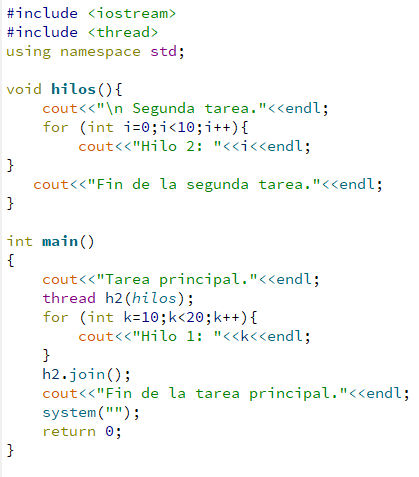
\includegraphics[width=0.48\textwidth]{1.png}
\caption{\label{fig1} Código de C++ en Qt.}
\end{figure}
\\
En este ejemplo se implementa un "Hilo 2"  haciendo uso de la clase thread.
\\
La clase thread, tras ser construida, generará un thread, sin necesidad de llamar a ningún método suyo.
\\
En el main se crea el hilo 2 e implementa un hilo 1 principal para evidenciar los resultados del comportamiento de ambos al momento de correr el programa.
\\
\begin{figure}[h!]
\centering
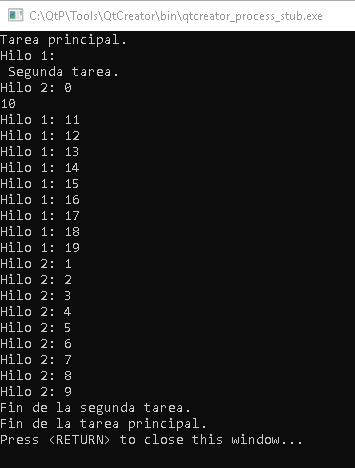
\includegraphics[width=0.48\textwidth]{2.png}
\caption{\label{fig1} Resultados.}
\end{figure}
\\
En los resultados se evidencia que el programa está ejcutando los dos hilos "simultáneamente", ejecuta una parte del hilo 1, luego una parte del hilo 2, vuelve al hilo 1 y por último regresa al hilo 2.
\\
\section{ANÁLISIS}
\\
\\
• Un hilo es una tarea que puede ser ejecutada al mismo tiempo que otra tarea.
\\
• Es más rápido cambiar de un hilo a otro dentro del mismo proceso, que cambiar de un proceso a otro.
\\
• El manejo de hilos está ligado al Hardware del equipo, según sus características se facilita la realización de diferentes procesos al mismo tiempo.
\\
• El sistema operativo solo reconoce un hilo de ejecución en el proceso.
\\
\\
\begin{thebibliography}{00}


\bibitem{b1}  Hilo (informática). (2020, 19 de junio). Wikipedia, La enciclopedia libre. Fecha de consulta: 20:56, julio 12, 2020 

\bibitem{b2} Que son los hilos de un procesador.(2019,03 de abril). profesionalreview, Fecha de consulta: 16:25, julio 12, 2020 

\bibitem{b3} Proyectos (Capitulos). (2019, 15 de agosto). Bibing. Fecha de consulta: 21:10, julio 12, 2020  

\bibitem{b4}  Hilo-implementaciones. (2020, 25 de abril). Wikipedia, Wiki. Fecha de consulta: 21:48, julio 16, 2020

\bibitem{b5}  Sistemas operativos-Recursos teóricos. (2014). fing.edu. Fecha de consulta: 21:30, julio 17, 2020 



\end{thebibliography}


\end{document}
